\documentclass[11pt,letterpaper]{article}
\usepackage[utf8]{inputenc}
\usepackage[T1]{fontenc}
\usepackage{lmodern}
\usepackage[margin=1in]{geometry}
\usepackage{microtype}
\usepackage{amsmath,amssymb,amsthm}
\usepackage{booktabs,array,tabularx}
\usepackage{graphicx,xcolor,url}
\usepackage[colorlinks=true,linkcolor=blue!45!black,citecolor=blue!45!black,urlcolor=blue!45!black]{hyperref}
\usepackage{caption}
\captionsetup{font=small,labelfont=bf}
\setlength{\parskip}{0.35em}
\setlength{\parindent}{0pt}
\setlength{\emergencystretch}{2em}
\renewcommand{\arraystretch}{1.15}
\newtheorem{proposition}{Proposition}
\newtheorem{theorem}{Theorem}
\title{Using Game Theory to Detect Fraud in AI-Assisted Banking\\[0.4em]\large Evidence Dependencies, Audit Disclosure, and Robust Verification in Agent-Assisted Banking}
\author{Prompted by Nariman Orujov\\[0.3em]\small All other work was carried out by AI agents.}
\date{26 October 2026\\\small Theoretical working paper with reproducible synthetic experiments}
\begin{document}
\maketitle

\begin{abstract}
Several AI agents can agree on a payment while relying on the same false evidence. Allocating additional reviews by agent identity can therefore overstate the independence of verification. This paper studies evidence-source auditing after mandatory transaction authorization. It represents overlapping attack routes and shared verification sources in a finite security game, allows the selected audit to be disclosed before the attacker commits, and optimizes against a specified set of reliability scenarios. The mathematical results establish an unbounded performance gap for a policy that mistakes repeated access to one source for independent checks, an exact three-regime audit policy in a worked disclosure example, and loss and regret bounds under estimation error. The computational study evaluates 600 synthetic settings derived from 100 evidence graphs, plus 300 finite-sample estimation experiments. In the specified scenario envelope, mean normalized worst-case loss is 0.655 for the robust policy and 0.741 for nominal optimization. These are model-based comparisons, not measured banking improvements. Outside the envelope, the robust policy performs worse than nominal optimization in 271 of 600 settings, illustrating the price and limits of robustness. The contribution is a source-explicit formulation, proved diagnostic results, and a fully reproducible assessment of when its guarantees hold. No language-model experiments, bank observations, or deployment claims are made.
\end{abstract}

\noindent\textbf{Keywords:} AI agents; evidence dependencies; transaction authorization; security games; robust optimization; audit disclosure.

\section{Introduction}

A payment recommendation may pass through an invoice reader, a supplier matcher, a ledger summarizer, and a contract reviewer. Their agreement can appear reassuring. Yet several recommendations may trace back to one supplier email or one unsupported summary. Counting those recommendations as independent support confuses the number of reviewers with the number of trustworthy observations.

The same problem can arise in the defense. Adding two auditors does not necessarily add two opportunities to discover a false claim. If both merely replay an identical source assessment, the second check repeats the first check's failure. The allocation problem must therefore describe what evidence a check can reveal, not just which agent performs it.

This paper asks: \emph{How should a bank allocate a limited number of independent evidence checks when checks overlap, evidence can fail jointly, and the attacker may learn the selected check?} The scope is deliberately specific. An external transaction service continues to enforce permissions, amount caps, approved beneficiaries, and request binding. The model addresses the business justification of a payment that survives these mandatory controls. It does not randomize permission enforcement.

The motivating workflow is hypothetical. The Bank of England and Financial Conduct Authority's 2024 survey reported AI use at 75\% of responding firms, but fully autonomous decisions in only 2\% of reported AI use cases \cite{boe2024}. Those figures describe that survey, not the current prevalence of autonomous banking. Existing studies nevertheless motivate examining agent compromise and the independence of evidence before increasing operational autonomy \cite{agentdojo,infection,mastrike,relay2026}.

The previous three-route allocation model is retained as an interpretable special case. The central analysis moves beyond it in three ways. First, audit schedules operate on identifiable sources, so repeated access and overlapping protection are explicit. Second, the attacker knows the policy and may also receive the selected schedule before choosing a route. Third, the defender may have several plausible loss matrices rather than one precisely known matrix.

\textbf{Contributions.} The paper provides (i) a source-based loss construction and a finite robust linear program with an explicit information sequence; (ii) proofs of an independence-blind allocation failure, disclosure-policy transitions, and estimation guarantees; and (iii) an executable synthetic study with independent primal--dual checks, strong comparison policies, component-removal comparisons, and an adverse scenario outside the design envelope. The finite-sample study additionally quantifies the cost of estimating the loss matrix.

These contributions do not establish the first audit game, the first leakage-aware security game, or the first demonstration that agent reports can be unreliable. The formulation combines established tools in a banking interpretation and develops explicit consequences of that combination. The paper's empirical claim is limited to completed synthetic computations. Its connection to language-model behavior remains a hypothesis requiring a separate experiment.

\section{Position relative to earlier work}

\subsection{Agent compromise and evidence dependence}

AgentDojo evaluates tool-using agents on both legitimate tasks and prompt-injection objectives, including e-banking tasks \cite{agentdojo}. Prompt Infection studies attacks propagating through agent communication \cite{infection}. MAStrike uses agent-level Shapley analysis to guide coordinated compromise and evaluates attacks in simulated workflows including finance \cite{mastrike}. These studies motivate the threat set; they do not supply the loss parameters used here. In particular, this paper does not reuse MAStrike's attack-success rates as banking risk estimates.

Arslan's \emph{Audit Without Verification} directly examines the danger of auditors relaying agent conclusions. It compares conclusions with underlying documentation and reports controlled interventions on the reports auditors receive \cite{relay2026}. That work already supports the need to distinguish an agent's conclusion from independently informative evidence. Our question concerns the allocation of scarce checks given an explicit model of which source can expose which harmful claim.

Zavattari, Tommasi, and Prencipe study audit-budget allocation across agent fleets under miscalibrated confidence and correlated errors \cite{fleet2026}. Their results make clear that limited auditing and correlated agent failures are already research topics. Here, the decision variables are distributions over evidence-source schedules; the adversary selects a harmful route, and the calculation includes schedule disclosure. The present experiments do not test confidence calibration or compare live agent fleets.

\subsection{Security games, strategic auditing, and disclosure}

Randomized defense against an adaptive attacker is established in security games \cite{securitygames}. Audit Games adds audit and punishment choices, and its multiple-resource extension treats restrictions on what resources can inspect \cite{auditgames,multiaudit}. Das, Yu, and Zhang study optimal auditing when strategic agents misreport information and collectively choose an equilibrium \cite{optimal2026}. Our agents are instruments or information-processing components in one attacker's strategy; they are not modeled as separate economic actors choosing a reporting equilibrium.

Xu and colleagues explicitly study information leakage about a realized defensive allocation \cite{leakage2015}. Consequently, neither leakage-aware optimization nor its expression as a linear program is claimed as new here. We use a restricted all-or-nothing disclosure channel to obtain a transparent closed-form example and combine it with source-level failure scenarios. The restriction is material: partial signals about individual checks require a richer information model.

\subsection{Authorization remains outside the optimization}

CaMeL separates trusted control from untrusted information and enforces data-use restrictions outside a vulnerable language model \cite{camel}. OWASP similarly recommends external tool authorization and transaction-specific server-side checks \cite{owaspagent,owasptransaction}. NIST identifies agent identity, delegation, and authority as implementation concerns \cite{nist2026}.

The present model adopts this separation. It supplies neither a replacement for these controls nor a demonstrated improvement over CaMeL. A payment that an existing reliable authorization rule already prevents has zero residual loss for that route. Additional auditing is relevant only to uncertainty that remains after those rules are enforced.

\section{Workflow, threat model, and evidence representation}

\subsection{Permitted actions can have false business justifications}

Consider an approved supplier receiving a payment within a valid spending mandate. Mechanical checks can establish that the supplier, account, amount, and approval are permitted. They do not automatically establish that the claimed goods arrived, that an invoice corresponds to a new obligation, or that a contract exception is authentic. These are candidate subjects for discretionary verification.

The six illustrative agent roles are the invoice reader, supplier matcher, ledger summarizer, anomaly reviewer, contract retriever, and exception reviewer. An attack route $C$ specifies a harmful claim and the subset of roles whose recommendations can be manipulated to support it. A route need not be a pair; the abstraction permits larger and overlapping coalitions. The computational suite uses six abstract routes, not measured vulnerabilities of these six roles.

\begin{table}[htbp]
\centering\small
\caption{Examples linking a residual claim to a verification source. These are workflow illustrations, not measured attack cases.}
\label{tab:workflow}
\begin{tabularx}{\textwidth}{@{}p{.24\textwidth}XX@{}}
\toprule
Residual claim & Potentially shared recommendation evidence & Additional source to inspect \\
\midrule
Goods were delivered & Supplier email copied into several agent summaries & Protected receiving record or authenticated confirmation \\
Charge is a new obligation & Reused payment-history summary & Original ledger entries and obligation identifiers \\
Exception permits the charge & Retrieved contract excerpt and forwarded exception note & Authoritative contract version and authenticated exception record \\
\bottomrule
\end{tabularx}
\end{table}

The model assumes initial influence over the allowed agent subset; it does not estimate the probability of obtaining that influence. One attack route is committed per modeled request. The execution gateway, audit scheduler, source-access controls, and audit-result enforcement remain outside attacker control. A source can still be incomplete, stale, or jointly unreliable under a specified scenario. Unrestricted compromise of the gateway is outside the threat model.

\subsection{Sources, checks, and residual loss}

Let $\mathcal C$ be a finite set of attack routes, $\mathcal A$ a set of available checks, and $\mathcal E$ a set of evidence sources. Check $a$ accesses source $e(a)$. A source means a distinct \emph{verification outcome}, not merely a hostname or document filename. Two readers replaying the same result share a source in this representation. If two inspections of one record can discover different inconsistencies, they should instead be represented by separate, possibly dependent outcomes.

For each route $C$, let $W_C\subseteq\mathcal E$ be the sources capable of exposing its false claim. A schedule $S\subseteq\mathcal A$ reaches
\begin{equation}
K_C(S)=W_C\cap\{e(a):a\in S\}.
\label{eq:sourceunion}
\end{equation}
The set operation is intentional: adding an alias of an already selected verification outcome does not create another independent observation.

Let $Z_e\in\{0,1\}$ indicate whether source $e$, if checked, yields a blocking inconsistency. A scenario $\theta$ specifies a joint distribution for $Z$ and a route severity $v_C\geq0$. For the factorized interpretation below, $Z$ is defined conditional on an otherwise harmful route outcome. Detection means that the gateway stops the action before harm. The residual expected loss is
\begin{equation}
L_\theta(C,S)=v_C\Pr_\theta\{Z_e=0\text{ for all }e\in K_C(S)\}.
\label{eq:sourceloss}
\end{equation}
The empty-set probability is one. The general game can instead accept a directly estimated residual-loss matrix if this source factorization is inappropriate. In particular, source effectiveness can depend on the route; separate route-conditional distributions can represent that dependence.

Equation~\ref{eq:sourceloss} permits arbitrary dependence between verification outcomes. The implemented generator uses a transparent special case: with probability $g_\theta$, all sources fail; otherwise their reveal indicators are independent with probabilities $d_{\theta e}$. It gives
\begin{equation}
L_\theta(C,S)=v_C\left[g_\theta+(1-g_\theta)
\prod_{e\in K_C(S)}(1-d_{\theta e})\right].
\label{eq:mixture}
\end{equation}
This is a generative assumption, not an estimated correlation between models. Repeating an identical outcome and sharing a common failure event are two different dependence mechanisms, both represented here.

\subsection{Hard budgets and the order of information}

Each check has nonnegative cost $c_a$. The admissible schedules are
\begin{equation}
\mathcal S_B=\left\{S\subseteq\mathcal A:\sum_{a\in S}c_a\leq B\right\}.
\label{eq:hardbudget}
\end{equation}
Thus every realized schedule respects the budget. All checks have unit cost in the reported suite. Unlike an expected-resource constraint, this definition cannot finance an oversized review by skipping another request. Queueing and latency remain separate operational requirements.

The defender commits to a distribution $x$ over $\mathcal S_B$. An adverse scenario $\theta$ is fixed for the request before the schedule is sampled. The attacker is conservatively assumed to know $\theta$ and $x$; the defender knows only the scenario set $\Theta$. The schedule $S\sim x$ is then drawn. Independently, a Bernoulli event with probability $\lambda$ reveals the complete schedule to the attacker. On the hidden branch, the attacker chooses a route without seeing $S$; on the disclosed branch, it chooses after seeing $S$. The source outcomes remain unobserved until verification. Audits are enforced before execution.

Independence of the disclosure event from $S$, $\theta$, and the source outcomes is essential. If expensive schedules leak more often, even the absence of disclosure conveys information. Equation~\ref{eq:disclosure} below would then be insufficient. Likewise, the attacker does not observe a source's realized success or failure before choosing its route.

\section{Robust auditing with possible disclosure}

\subsection{Objective and finite linear program}

Write $M_{\theta S}=\max_C L_\theta(C,S)$. Conditional on $\theta$, the attacker's maximum expected loss is
\begin{equation}
F_{\theta,\lambda}(x)=(1-\lambda)\max_C\sum_Sx_SL_\theta(C,S)
+\lambda\sum_Sx_SM_{\theta S}.
\label{eq:disclosure}
\end{equation}
The first term chooses one route before observing the schedule; the second permits a different best route for each revealed schedule. Taking a maximum over routes after averaging in both branches would understate the value of disclosure.

The defender minimizes $\max_{\theta\in\Theta}F_{\theta,\lambda}(x)$. Define
$A_{(\theta,C),S}=(1-\lambda)L_\theta(C,S)+\lambda M_{\theta S}$.
The resulting program is
\begin{equation}
\begin{aligned}
\text{minimize}_{x,t}\quad &t\\
\text{subject to}\quad &\sum_S A_{(\theta,C),S}x_S\leq t
&&\text{for every }\theta,C,\\
&\sum_Sx_S=1,\qquad x_S\geq0.
\end{aligned}
\label{eq:robustlp}
\end{equation}
This is a standard finite matrix-game linear program. The contribution is the specification of its entries and information assumptions, not a new LP algorithm. Its dual supplies a certificate: find weights $q_{\theta C}\geq0$ summing to one that maximize $u$, subject to $\sum_{\theta,C}q_{\theta C}A_{(\theta,C),S}\geq u$ for every schedule. A primal upper bound and dual lower bound that agree verify the finite optimization independently of a solver's success flag.

\subsection{What the robustness guarantee covers}

The scenario set is a modeling commitment. It does not become credible merely because the optimization considers its worst member. A scenario may describe a compromised record service, weaker inspection accuracy, or different severity assumptions. The solution protects against the specified loss matrices and also against their convex mixtures: for $\bar L=\sum_\theta w_\theta L_\theta$, maxima are convex, so
$F_{\bar L,\lambda}(x)\leq\sum_\theta w_\theta F_{\theta,\lambda}(x)\leq\max_\theta F_{\theta,\lambda}(x)$.
This statement does not cover arbitrary interpolation of source probabilities, because Equation~\ref{eq:mixture} is nonlinear in those probabilities.

The scenario is fixed before the realized schedule. Allowing an adversary to choose a new scenario after seeing each schedule produces a different, stronger uncertainty model. The present LP should not be advertised as covering that setting.

The number of schedules can grow exponentially. With $a$ checks and an integer unit-cost budget $B$, there are $\sum_{j=0}^{B}\binom{a}{j}$ schedules and $|\Theta||\mathcal C|$ game rows. Enumeration is suitable for the small study here. Large deployments would require structural simplification or additional optimization methods; no scalability claim is made.

\section{Analytical results}

\subsection{Repeated evidence can make an allocation arbitrarily poor}

\begin{theorem}[Failure of independence-blind allocation]
\label{thm:aliases}
For any integer budget $k\geq1$ and probabilities $0<q<p<1$, there is a one-route instance in which the policy optimized under false check independence has actual residual loss $(1-q)^{-(k-1)}$ times the source-aware optimum. The ratio is unbounded as $k$ grows.
\end{theorem}

\begin{proof}
Normalize unaudited loss to one. Provide $k$ check labels that all replay a single source with reveal probability $p$, plus $k-1$ other sources with independent reveal probability $q$. Every check costs one. A calculation that treats labels as independent assigns residual loss $(1-p)^k$ to inspecting all $k$ aliases. Since $p>q$, that is its unique optimal source composition. Its actual loss is $1-p$, because all selected checks share one outcome. A correct allocation selects one alias and all $k-1$ independent alternatives, with loss $(1-p)(1-q)^{k-1}$. No other schedule can improve this product: repeating a source adds no revelation, and the $p$ source is more informative than any $q$ source. Dividing the two losses gives the stated ratio.
\end{proof}

For $p=0.9$, $q=0.8$, and $k=4$, the independence-blind allocation predicts loss $0.0001$ but actually incurs $0.1$. The source-aware allocation incurs $0.0008$, a factor of 125 lower in this constructed example. This is an existence result, not a claim that operational banks exhibit that factor. It isolates a failure that cannot be repaired by optimizing the wrong matrix more accurately.

There is also a direct protection floor. If, for route $C$, an event of probability $\rho_C$ prevents every admissible source from revealing the inconsistency, every schedule has loss at least $v_C\rho_C$. Consequently, any hidden or disclosed policy has worst loss at least $\max_C v_C\rho_C$. Under Equation~\ref{eq:mixture}, $g_\theta v_C$ is one such floor. Scheduling cannot create missing evidence.

\subsection{The price of audit disclosure}

\begin{proposition}[Disclosure value for a known loss matrix]
\label{prop:leakage}
For a fixed finite loss matrix with entries in $[0,V]$, let
$V_\lambda=\min_x F_\lambda(x)$ over hard-budget schedules. Then $V_\lambda$ is nondecreasing, concave, and piecewise linear in $\lambda$. Moreover,
$V_0\leq V_\lambda\leq V_1=\min_S\max_C L(C,S)$ and
$V_\lambda-V_0\leq\lambda V$.
\end{proposition}

\begin{proof}
For a fixed $x$, write $a(x)=\max_C\sum_Sx_SL(C,S)$ and
$b(x)=\sum_Sx_S\max_C L(C,S)$. Then $0\leq b(x)-a(x)\leq V$, and $F_\lambda(x)=a(x)+\lambda[b(x)-a(x)]$. Monotonicity follows pointwise; taking the infimum of affine functions of $\lambda$ gives concavity. A finite LP with an objective affine in $\lambda$ has finitely many relevant vertices, giving piecewise linearity. At $\lambda=1$ the objective is linear in $x$, so a pure admissible schedule is optimal. Evaluating a $\lambda=0$ optimizer at $\lambda>0$ proves the last bound.
\end{proof}

The known-matrix qualification matters. Under scenario uncertainty, mixing can remain useful even with full disclosure: two scenarios with one route each and loss rows $(0,1)$ and $(1,0)$ have robust mixed value $1/2$, while either fixed schedule has robust loss one. The randomization then hedges scenario uncertainty; it no longer hides the schedule from the attacker.

\subsection{An exact three-regime example}

Take three routes with losses $(80,60,40)$ and a relevant audit that prevents 90\% of harmful outcomes. Exactly one route is audited. If $p_j$ is its selection probability, hidden loss is
\begin{equation}
r_j(p_j)=v_j(1-0.9p_j),\qquad p_1+p_2+p_3=1.
\label{eq:small}
\end{equation}
The no-disclosure minimax allocation is $(67,46,4)/117$ with value $504/13=38.77$. Uniform allocation gives loss 56.00, so the familiar 30.77\% reduction is recovered for these assumed inputs.

Disclosure changes the optimization, not just the reported risk. The losses after revealing audits 1, 2, and 3 are respectively $(60,80,80)$. An optimal allocation is
\begin{equation}
p^*(\lambda)=
\begin{cases}
(67,46,4)/117,&0\leq\lambda<27/52,\\
(17,10,0)/27,&27/52<\lambda<27/37,\\
(1,0,0),&27/37<\lambda\leq1.
\end{cases}
\label{eq:thresholds}
\end{equation}
At a threshold, convex combinations of the adjacent allocations are optimal. The value is the lower envelope
\begin{equation}
V_\lambda=\min\left\{
\frac{504}{13}+\frac{3484}{117}\lambda,
40+\frac{740}{27}\lambda,
60\right\}.
\label{eq:envelope}
\end{equation}
Appendix~\ref{app:thresholds} derives the transitions. They occur at disclosure probabilities approximately 0.519 and 0.730. Retaining the original policy under full disclosure gives 68.55, while reoptimization gives 60.00. Thus disclosure need not immediately eliminate randomization, but eventually changes which policy is best in this instance.

\subsection{Estimation error and auditable certificates}

\begin{proposition}[Uniform error and policy regret]
\label{prop:errors}
Suppose true and estimated loss matrices share the same route, scenario, and schedule sets, all entries lie in $[0,V]$, and
$\max_{\theta,C,S}|L_\theta(C,S)-\widehat L_\theta(C,S)|\leq\epsilon$.
If $|\lambda-\widehat\lambda|\leq\eta$, then every policy's robust objective changes by at most $\epsilon+\eta V$. A policy optimized for $(\widehat L,\widehat\lambda)$ has true excess loss over the true optimum at most $2(\epsilon+\eta V)$.
\end{proposition}

\begin{proof}
Taking a maximum and taking a probability-weighted average are each 1-Lipschitz in the uniform norm. Both branches in Equation~\ref{eq:disclosure} therefore change by at most $\epsilon$; their convex combination has the same bound. Changing $\lambda$ contributes at most $\eta V$ by the bound on $b(x)-a(x)$. A maximum over scenarios preserves the bound. Apply it once at the estimated optimizer and once at the true optimizer, using optimality under the estimated model between the two steps.
\end{proof}

This is a deterministic stability result. It does not assert that the required uniform accuracy is available. A simple statistical route is possible when every one of $K=|\Theta||\mathcal C||\mathcal S_B|$ cells has $n$ independent bounded observations with mean $L_\theta(C,S)$ and range $[0,V]$. Hoeffding's inequality and a union bound give, with probability at least $1-\delta$,
\begin{equation}
\epsilon_n=V\sqrt{\frac{\log(2K/\delta)}{2n}}.
\label{eq:hoeffding}
\end{equation}
The concentration inequality is standard \cite{hoeffding}. It assumes independent draws within each cell; correlations between different cells do not invalidate the union bound. A shared task template can invalidate the within-cell sampling assumption if repeated runs are treated as independent evidence about a wider task population.

When $\lambda$ is known, set $U_\theta(C,S)=\min\{V,\widehat L_\theta(C,S)+\epsilon_n\}$. Monotonicity implies that optimizing with $U$ gives an upper certificate for its selected policy whenever all true entries lie below $U$. The certificate accounts for selecting the policy using the same estimates because the event is uniform over cells. If only an upper bound on $\lambda$ is known, use that upper bound as well. A certificate is conditional on the fixed threat set and sampling assumptions; it cannot cover an omitted attack route.

\section{Completed computational study}

\subsection{Design and reproducibility}

The suite contains 100 generated evidence graphs, each evaluated at budgets $B\in\{1,2\}$ and disclosure probabilities $\lambda\in\{0,0.25,0.5\}$, giving 600 settings. These are six parameter settings per graph, not 600 independent observations of banking systems. Every graph has six routes, five sources, and seven check labels with source map $(0,0,1,1,2,3,4)$. The two pairs of aliases test repeated evidence. Each route receives either two or three uniformly chosen distinct eligible sources, with equal probability for the two sizes. Route losses are independently drawn as integers from 30 through 100. Initial source reveal probabilities are independently uniform on $[0.65,0.95)$.

Three design scenarios are used. In the nominal scenario, common failure is 0.03. In scenario A, reveal probabilities for sources 0 and 1 are multiplied by 0.35 and common failure is 0.15. In scenario B, the same multiplier applies to sources 2 through 4 and common failure is 0.15. These two adverse scenarios cross in their relative source quality, creating a meaningful allocation tradeoff. The values are explicit stress assumptions; they are not measured rates or a calibrated banking distribution.

The master seed is 20261026; graph $i$ uses a NumPy generator initialized with seed $20261026+i$. The stored \texttt{instances.json} records every generated input. There are eight schedules at budget one and 29 at budget two, including the empty schedule. Losses are evaluated exactly from Equation~\ref{eq:mixture}, rather than estimated by attack sampling. The same input instance is used for every comparison policy.

Two additional evaluations are kept out of policy fitting. One uses the loss-matrix mixture $0.2L_0+0.4L_A+0.4L_B$, which must lie within the robust guarantee. The other uses common failure 0.35 and multiplies the original reveal probabilities of sources 0 and 2 by 0.15. This second scenario is an intentionally omitted adverse condition; it is not assumed to belong to the convex hull. Neither evaluation is a holdout of real language-model behavior.

\subsection{Comparison policies and attribution}

All policies share the same hard schedule budget and loss objective at evaluation. \emph{Uniform distinct sources} samples uniformly among size-$B$ source combinations, using one check representative per source. It therefore avoids wasting capacity on aliases. \emph{Best fixed robust schedule} exhaustively chooses the pure schedule minimizing worst loss over the three scenarios; it is a stronger baseline than always inspecting the initially highest-loss route. \emph{Nominal minimax} optimizes only the nominal matrix. \emph{Average-scenario minimax} optimizes the arithmetic mean matrix, imposing equal scenario weights rather than worst-scenario protection.

Two comparisons remove a modeling component. The \emph{independent-check ablation} retains each check's marginal detection rate $(1-g_\theta)d_{\theta e}$ but multiplies failure rates over check labels, incorrectly treating aliases and common failures as independent. It still optimizes over all three scenarios and uses the correct disclosure probability. The \emph{hidden-selection ablation} uses the correct source model and scenario set but optimizes as if $\lambda=0$. Finally, \emph{source-aware robust} uses Equation~\ref{eq:robustlp} with the stated $\lambda$.

All optimized policies receive the exact matrices of the model they are permitted to use. Thus this experiment isolates modeling and objective choices; it does not measure how hard those matrices are to learn. The separate sampling experiment addresses one simplified estimation regime.

\subsection{Results within and outside the scenario envelope}

\begin{table}[htbp]
\centering\small
\caption{Results over 600 synthetic settings. Envelope and Outside are mean losses divided by the largest route loss within each setting. Median gap and 95th gap are the median and 95th percentile of excess loss over the robust optimum, in unnormalized assumed units. Outside uses the omitted adverse scenario.}
\label{tab:results}
\begin{tabular}{@{}lrrrr@{}}
\toprule
Policy & Envelope & Median gap & 95th gap & Outside \\
\midrule
Uniform distinct sources & 0.791 & 12.05 & 20.27 & 0.815 \\
Best fixed (robust) & 0.740 & 6.30 & 20.37 & 0.751 \\
Nominal minimax & 0.741 & 6.72 & 18.85 & 0.731 \\
Average-scenario minimax & 0.723 & 5.02 & 15.70 & 0.716 \\
Independent-check ablation & 0.660 & 0.00 & 3.45 & 0.732 \\
Hidden-selection ablation & 0.660 & 0.00 & 2.76 & 0.736 \\
Source-aware robust & 0.655 & 0.00 & 0.00 & 0.730 \\
\bottomrule
\end{tabular}

\end{table}

The robust policy has mean normalized envelope loss 0.655, compared with 0.741 for nominal optimization and 0.791 for uniform distinct-source sampling. A lower value is better. Its advantage on the exact objective it optimizes is expected by construction; this comparison is not evidence of an operational breakthrough. The useful diagnostics are the size of the model-mismatch penalties, the circumstances where components matter, and the cost paid elsewhere.

At budget one, the independence ablation is exact because only one check is selected. At budget two, it produces strictly higher true envelope loss in 263 of 300 settings, with mean excess 0.94 units and maximum excess 10.00. Across all 600 settings, its reported bound understates its true envelope loss in 275 settings. The ablation combines ignored alias dependence and ignored common failures; the theorem isolates the alias mechanism, but this aggregate comparison does not assign the entire gap to aliases alone.

Ignoring disclosure gives positive excess loss in 244 of 600 settings, with the largest observed gap 8.24 units. The zero-disclosure settings necessarily show no penalty. Reporting a pooled median of zero without these qualifications would conceal meaningful failure cases.

Robustness has a cost. The mean increase in nominal-scenario loss relative to the nominal optimizer is 10.26 assumed units. In the omitted adverse scenario, robust optimization performs worse than nominal optimization in 271 of 600 settings. Its design-envelope value is exceeded in 430 settings. Average-scenario optimization has lower \emph{mean} outside loss than robust optimization in this particular omitted scenario (0.716 versus 0.730). These outcomes are retained because they show that protection against a specified envelope is not protection against every possible failure.

Every policy's loss under the held-out convex mixture remains below its own worst-envelope loss, as required by the convexity argument. This is an implementation check and an illustration of the guarantee's domain, not a test of extrapolation to new evidence mechanisms.

\begin{figure}[htbp]
\centering
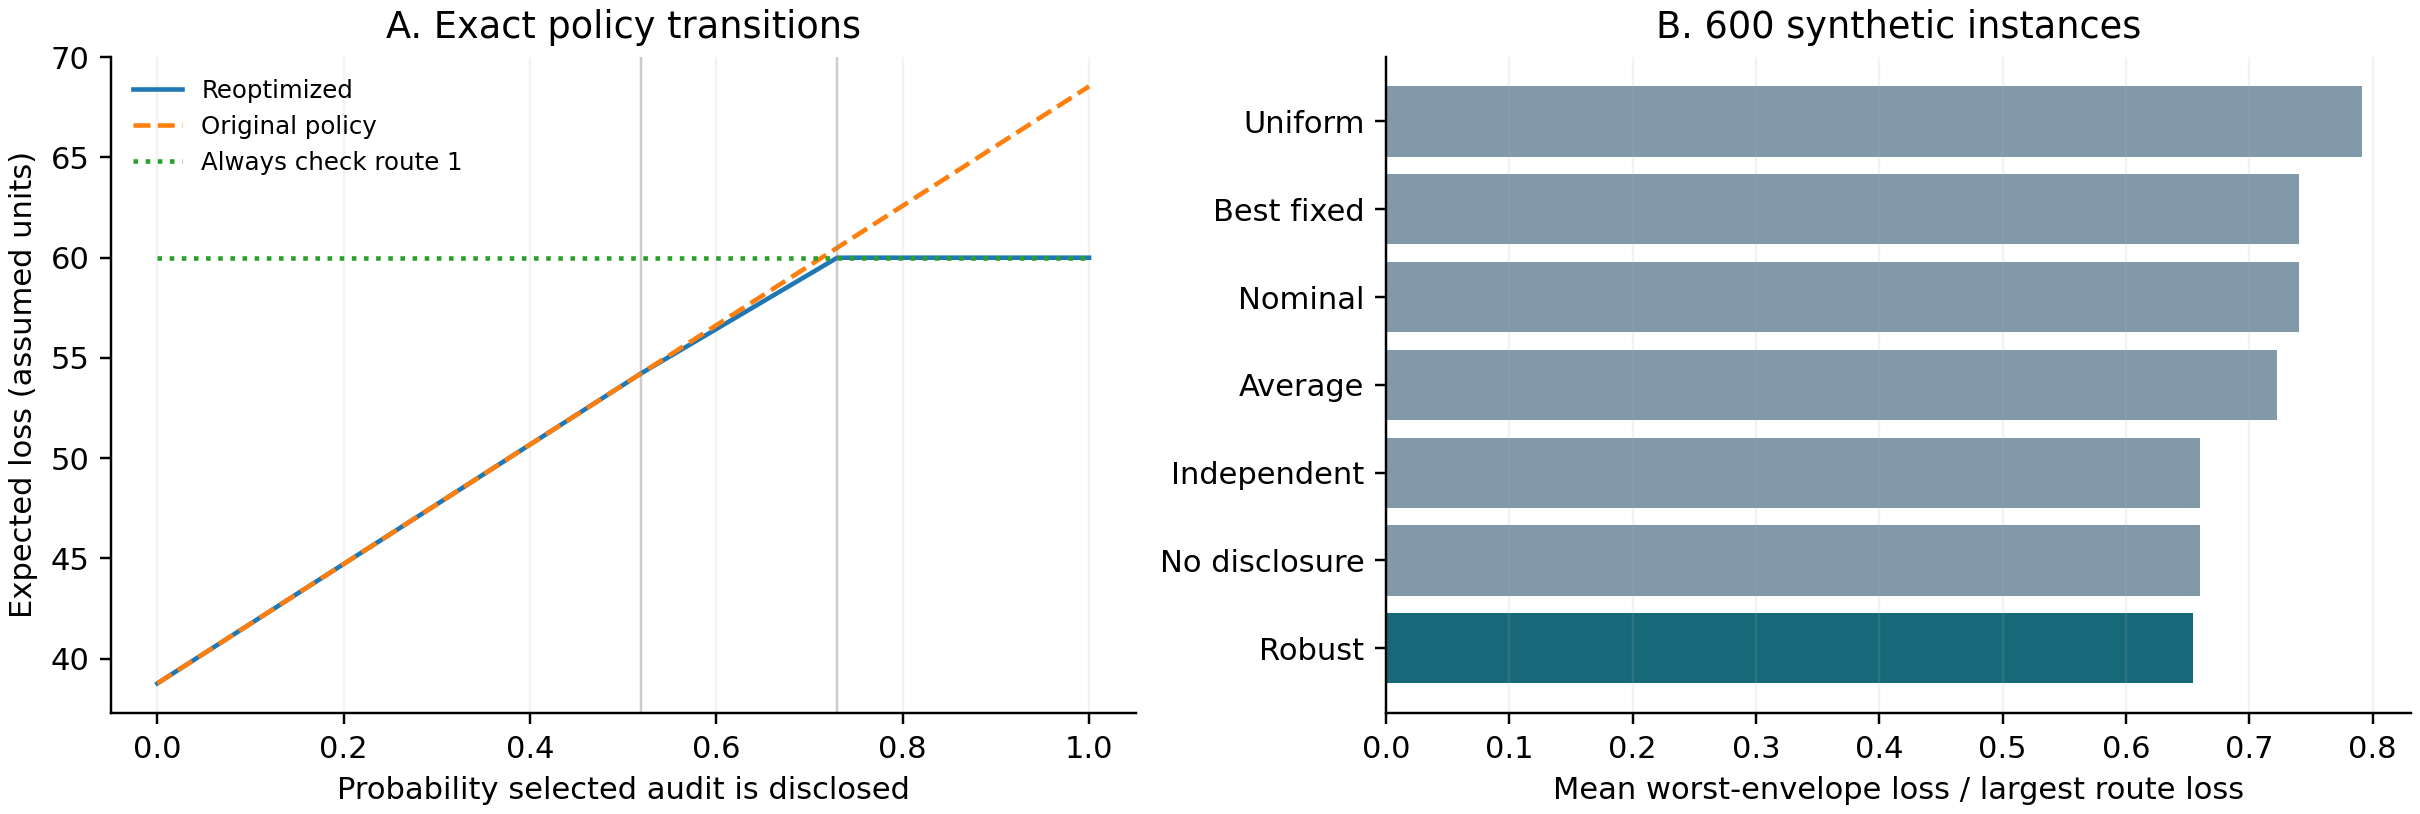
\includegraphics[width=\textwidth]{results/extended/extended_results.png}
\caption{Completed synthetic calculations. Left: exact disclosure transitions in the three-route example. Right: mean normalized worst-envelope loss over the 600 settings. The two panels use different constructions and should not be interpreted as measurements of bank fraud.}
\label{fig:results}
\end{figure}

\subsection{Finite-sample estimation experiment}

For each of the 100 graphs, fix $B=2$ and $\lambda=0.25$. Estimate each of the $K=3\times6\times29=522$ matrix entries from $n\in\{50,200,1000\}$ independent Bernoulli harmful-outcome draws, scaled by its route loss. This gives 300 synthetic estimation experiments. The draws are generated through binomial counts; there are no language-model calls. Each setting uses a separate deterministic random stream, specified in the code. Optimize both the empirical matrix and the conservative upper matrix with $\delta=0.05$. Evaluate their policies using the exact underlying synthetic matrices.

\begin{table}[htbp]
\centering\small
\caption{Synthetic loss-matrix estimation. Regret is the empirical-matrix policy's true robust excess loss, normalized by $V=\max_Cv_C$. Coverage counts settings where the upper-matrix policy's reported bound covers its true loss. Total draws are per graph, not across the entire suite.}
\label{tab:sampling}
\begin{tabular}{@{}rrrrr@{}}
\toprule
$n$ per cell & Total draws & Mean regret/$V$ & Max regret/$V$ & Bound coverage \\
\midrule
50 & 26,100 & 0.0319 & 0.1408 & 100/100 \\
200 & 104,400 & 0.0117 & 0.0573 & 100/100 \\
1000 & 522,000 & 0.0058 & 0.0189 & 100/100 \\
\bottomrule
\end{tabular}

\end{table}

Mean normalized plug-in regret falls from 0.0319 at $n=50$ to 0.0058 at $n=1000$. All 300 upper certificates cover the corresponding true loss in this run. This is consistent with a conservative simultaneous bound; it does not establish universal or exactly 95\% empirical coverage. The deterministic $2\epsilon$ regret bound is also checked using the realized largest cell error, separately from the probabilistic confidence radius.

The cost is substantial: $n=1000$ represents 522,000 cell observations per graph. The generic bound has $\epsilon_n/V\approx0.0705$ at that sample size, so the certified regret ceiling $2\epsilon_n/V\approx0.141$ is much larger than the observed mean regret. Naive full-matrix estimation is therefore an expensive route to useful guarantees. Sharing information across structured sources could reduce the burden, but requires a separate argument about estimation error and misspecification. The current experiment does not provide that argument.

\subsection{Verification and interpretation}

The implementation independently solves the defender LP and attacker dual for all 4,523 optimizations in the extended run. The largest primal--dual gap is below $3\times10^{-10}$ and the largest probability-feasibility error below $3\times10^{-12}$. Additional checks enumerate every binary source state for a reference instance, test duplicate-source invariance, exhaustively verify the alias counterexample for budgets one through six, compare the exact disclosure solution with 103 LP evaluations, and check the perturbation bounds on independently generated matrices.

These checks substantiate the formulas and their implementation. They do not validate the scenario distribution. Tables report exact values or descriptive summaries of the specified generated suite. Confidence intervals about real-world fraud would be inappropriate. The 95th percentile column describes dispersion within this finite suite, while the probability guarantee in Equation~\ref{eq:hoeffding} concerns the separately defined synthetic observation model.

\section{Implementation requirements and empirical validation}

\subsection{What must be trusted in a working system}

A practical implementation needs an external gateway that binds each proposal, verification outcome, and approval to the same transaction version. Changes to amount, beneficiary, or material claims require appropriate revalidation. Audit scheduling, source identifiers, and blocking outcomes must be protected from the agents under review. Mandatory checks always apply, including when no discretionary audit is selected.

The evidence map cannot simply be accepted from an attacker-controlled summary. It should be reconstructed from protected retrieval logs, record identifiers, and explicit verification-service interfaces. Provenance establishes where information came from; it does not prove that the information is correct. The uncertainty model must still represent stale records, shared upstream errors, and unavailable corroboration. If provenance itself is forged, the source model may be wrong before optimization begins.

A hard check-count cap does not guarantee a deadline or limit false holds. An implemented scheduler must also respect check duration, staffing, and escalation policy. The present loss matrix counts harmful outcomes only. Legitimate-payment delays and rejected legitimate tasks need explicit costs or constraints before an operational policy can be chosen.

\subsection{A concrete next experiment, not a completed result}

The next study should implement the six agent roles with real language models in a sandbox containing synthetic invoices, delivery records, contract versions, and a ledger. Mandatory authorization should be a deterministic external service. The evaluation must distinguish legitimate authorized tasks, requests that mandatory controls should reject, and permitted actions supported by false business evidence.

A direct hypothesis is that source-aware scheduling reduces executed harmful payments relative to a source-independent policy at a matched review cost, particularly when several agents share evidence. A second hypothesis is that adapting to observed disclosure improves protection when the schedule leaks. These are hypotheses to test, not claims established by the present computation.

Cases should be split by document template, supplier, and attack family before estimating parameters or tuning policies. Development cases determine the evidence model, scenario set, and operating point. All choices should then be frozen for a held-out evaluation. Auditors must receive realistic evidence, including missing or ambiguous records, rather than access to the evaluator's hidden ground truth. Success should be scored from executed ledger changes and authorization state, following the task-and-security distinction in agent benchmarks \cite{agentdojo}.

Comparisons should include mandatory controls alone, a tuned conventional risk-based policy, uniform source coverage, nominal and robust scheduling, and full independent review as a higher-cost reference. Attackers should receive matched optimization budgets and adapt separately to each defense. Several model families and repeated runs should be used, with model versions and prompts recorded. Sample size should follow a pilot estimate of variability and a prespecified practically meaningful effect, rather than an arbitrary target number of runs.

The primary outcomes should include harmful payments executed and legitimate tasks completed; secondary outcomes should include false holds, latency, review effort, and API cost. Intervals should account for shared templates and paired cases. Reporting the largest observed attack-family loss does not certify an unrestricted worst-case guarantee. A practitioner review of the payment workflow can assess plausibility, but does not replace measured security evaluation.

\section{Limitations}

The main limitation is the absence of live-agent or banking experiments. All source probabilities, severity values, graph structures, and adverse scenarios are designed inputs. The results cannot support a claim that banks would reduce fraud by a particular percentage. Even the three-route 30.77\% improvement is a property of its stipulated game.

Source identification is assumed correct. Perfectly repeated outcomes justify alias collapse, but repeated inspections can sometimes add independent information. Incorrectly collapsing such inspections can discard useful protection; incorrectly separating identical outcomes can produce the failure in Theorem~\ref{thm:aliases}. Estimating which case applies is an empirical problem.

The attacker chooses one route per request, is loss-maximizing, and has the information described in the threat model. Repeated interactions, attack cost, deterrence, simultaneous fraud, and learning the audit policy over time are omitted. The all-or-nothing disclosure channel is intentionally simple. A joint change in source quality and disclosure can violate its independence assumptions.

The robust envelope is finite and chosen by the analyst. The omitted-scenario experiment demonstrates its limits rather than resolving them. Normalized conditional loss does not estimate annual financial loss or attack prevalence. False alarms, customer friction, institutional coverage requirements, and unequal check costs are not evaluated in the suite, although some can be represented by further constraints or richer payoffs.

Finally, the formal tools are established and the instances are small. The work's value rests on explicit source modeling, diagnostic proofs, reproducibility, and visible failure conditions. Broader algorithmic novelty, scalable optimization, and practical superiority require additional research.

\section{Conclusion}

The independence of verification is a property of evidence and failure mechanisms, not of the number of agent names in a workflow. A source-explicit audit game makes that distinction operational: it identifies what each schedule can discover, which failures it shares, and what the attacker knows before committing.

The analytical results show how false independence can produce an unbounded allocation gap, how disclosure changes optimal randomization, and how uniform estimation errors translate into policy regret. The completed synthetic study confirms these mechanisms in finite models and exposes the cost of robustness outside its design envelope. Together they support a precise, limited claim: evidence dependencies and attacker information should be specified before an audit allocation is called protective. Whether the resulting policies improve actual agent-assisted banking remains a question for the proposed empirical study.

\section*{Contribution and AI disclosure}

Nariman Orujov prompted this work. All other aspects of the work and paper preparation were carried out by AI agents.

\section*{Data and code availability}

\texttt{analysis/evidence\_audit.py} generates the extended study, certificates, tables, and figure. The directory \texttt{results/extended/} contains all 100 input graphs, 4,200 policy-result rows, 300 sampling-result rows, the disclosure curve, summary statistics, and a SHA-256 manifest. \texttt{analysis/audit\_game.py} retains the original three-route calculation. \texttt{REPRODUCING.txt} records dependencies, commands, and the distinction between completed work and future experiments. The source package contains no bank records, credentials, or external model calls. No external repository or publication status is asserted.

\bibliographystyle{unsrt}
\bibliography{references}

\appendix
\section{Derivation of the disclosure thresholds}
\label{app:thresholds}

Let $t=\max_jr_j(p_j)$. For a feasible bound $t$, the minimum probabilities on routes 2 and 3 are
$p_2\geq\max\{0,(60-t)/54\}$ and
$p_3\geq\max\{0,(40-t)/36\}$.
Because disclosed loss is $80-20p_1$, the best feasible policy for a specified $t$ maximizes $p_1$. On $504/13\leq t\leq40$, this gives
$p_1=-11/9+5t/108$ and disclosed loss $940/9-25t/27$.
The combined objective is therefore
$\lambda940/9+t(1-52\lambda/27)$.
It is minimized at the lower or upper endpoint according to whether $\lambda$ is below or above $27/52$.

For $40\leq t\leq60$, choose $p_3=0$,
$p_2=(60-t)/54$, and $p_1=-1/9+t/54$.
Disclosed loss is $740/9-10t/27$, and combined loss is
$\lambda740/9+t(1-37\lambda/27)$.
The endpoint changes at $\lambda=27/37$.
Values $t>60$ cannot improve on always inspecting route 1, which gives loss 60 on both branches. The endpoint policies are exactly those in Equation~\ref{eq:thresholds}; substituting them yields Equation~\ref{eq:envelope}.

The starting value $504/13$ follows from equalizing the three hidden residuals with a one-check budget. An independent lower certificate is the attacker mixture $(3,4,6)/13$, which gives expected loss $504/13$ against every pure one-route audit. This verifies the hidden optimum without relying on the numerical solver.

\section{Experimental audit trail}
\label{app:trail}

All extended runs used Python 3.14.4, NumPy 2.5.4, and SciPy 1.17.1 with the HiGHS linear-programming backend. Plotting used Matplotlib 3.10.7 with distribution packaging. The suite ran in approximately seven seconds in the supplied environment; this is an execution record, not a hardware-normalized performance benchmark. Numerical tables are generated from the same result objects as the machine-readable outputs.

The seven policies are evaluated once per graph, budget, and disclosure setting. The independent-check model is deliberately misspecified; its underestimated guarantee is reported as an error, not substituted for true evaluation. The source-aware policy receives no access to the omitted adverse scenario. An oracle optimized for that scenario is computed only for diagnostics and retained in the raw CSV.

The concentration experiment draws each cell's sample count independently conditional on its generated matrix. It therefore satisfies the within-cell assumptions used in the proof by construction. It does not establish that traces from repeated language-model workflows satisfy those assumptions.

\end{document}
